% =====================================================================
% AI Academy -- National AI Center
% Software Engineering Final Project -- Team Report
% Team1 -- Topic 4: Async Research Assistant
%
% Build:  tectonic report.tex        (or pdflatex report.tex, twice)
% =====================================================================

\documentclass[11pt,a4paper]{article}

\usepackage[dvipsnames]{xcolor}
\definecolor{accent}{HTML}{0B3D91}
\definecolor{accent2}{HTML}{8B0000}
\definecolor{soft}{HTML}{F2F4F8}
\definecolor{okgreen}{HTML}{166534}

% ===== CONFIGURATION =================================================
\newcommand{\teamname}{Team1}
\newcommand{\topicchoice}{Topic 4 --- Async Research Assistant}
\newcommand{\member}[2]{\textbf{#1} (\texttt{#2})}
\newcommand{\reportdate}{19 September 2026}
\newcommand{\repolink}{\href{https://github.com/Nurana100/team1-ai-eng-research-assistant}%
{\texttt{github.com/Nurana100/\allowbreak team1-ai-eng-research-assistant}}}

\newcommand{\coursecode}{AI-ENG-110}
\newcommand{\coursename}{Software Engineering}
\newcommand{\institution}{AI Academy, National AI Center}
\newcommand{\semester}{Spring 2026}

% ===== PACKAGES ======================================================
\usepackage[margin=2.2cm,headheight=15pt]{geometry}
\usepackage[T1]{fontenc}
\usepackage[utf8]{inputenc}
\usepackage[final,protrusion=true,expansion=false]{microtype}
\usepackage{amsmath,amssymb}
\usepackage{graphicx}
\usepackage{booktabs}
\usepackage{array}
\usepackage{tabularx}
\usepackage{ragged2e}
\usepackage{enumitem}
\usepackage[parfill]{parskip}
\usepackage{listings}
\usepackage[most]{tcolorbox}
\usepackage{titlesec}
\usepackage{fancyhdr}
\usepackage{lastpage}
\usepackage{tikz}
\usetikzlibrary{shapes.geometric,arrows.meta,positioning,fit,backgrounds}
\usepackage[hidelinks]{hyperref}

\emergencystretch=4em
\hbadness=10000
\hfuzz=2pt
\sloppy

\hypersetup{
  colorlinks=true,
  linkcolor=NavyBlue,
  urlcolor=NavyBlue,
  citecolor=NavyBlue,
  pdftitle={\coursecode\ Final Project Report -- Team1},
  pdfauthor={Team1}
}

\titleformat{\section}
  {\Large\bfseries\color{accent}}{\thesection.}{0.6em}{}
\titleformat{\subsection}
  {\large\bfseries\color{accent}}{\thesubsection}{0.5em}{}
\titlespacing*{\section}{0pt}{1.4ex plus .3ex minus .2ex}{1.0ex plus .2ex}
\titlespacing*{\subsection}{0pt}{1.2ex plus .3ex minus .2ex}{0.7ex plus .2ex}
\setlength{\parskip}{0.42\baselineskip}

\newtcolorbox{keybox}[1]{
  colback=soft, colframe=accent, boxrule=0.6pt,
  arc=2pt, left=8pt, right=8pt, top=5pt, bottom=5pt,
  title={\small\bfseries #1}, coltitle=white, colbacktitle=accent,
  fonttitle=\bfseries
}

\definecolor{codegreen}{rgb}{0,0.55,0}
\definecolor{codegray}{rgb}{0.4,0.4,0.4}
\definecolor{codepurple}{rgb}{0.55,0,0.78}
\definecolor{backcolour}{rgb}{0.97,0.97,0.97}

\lstdefinestyle{python}{
  language=Python,
  backgroundcolor=\color{backcolour},
  commentstyle=\color{codegreen},
  keywordstyle=\color{accent},
  numberstyle=\tiny\color{codegray},
  stringstyle=\color{codepurple},
  basicstyle=\ttfamily\footnotesize,
  breakatwhitespace=false,
  breaklines=true,
  keepspaces=true,
  numbers=left,
  numbersep=6pt,
  tabsize=2,
  frame=single,
  framerule=0.4pt,
  rulecolor=\color{black!30},
}

\lstdefinestyle{plain}{
  backgroundcolor=\color{backcolour},
  basicstyle=\ttfamily\footnotesize,
  breaklines=true,
  keepspaces=true,
  numbers=none,
  frame=single,
  framerule=0.4pt,
  rulecolor=\color{black!30},
}

\pagestyle{fancy}
\fancyhf{}
\fancyhead[L]{\small\textit{\coursecode\ -- Final Report -- \teamname}}
\fancyhead[R]{\small\textit{\semester}}
\fancyfoot[L]{\small\textit{\institution}}
\fancyfoot[R]{\small Page \thepage\ of \pageref{LastPage}}
\renewcommand{\headrulewidth}{0.4pt}
\renewcommand{\footrulewidth}{0.4pt}

% =====================================================================
\begin{document}

\begin{center}
{\small \textsc{\institution} \\[0.2em] \textsc{\coursecode\ -- \coursename\ -- \semester}}\\[1.2em]
{\Large\bfseries\color{accent} Final Project Report}\\[0.3em]
{\LARGE\bfseries \topicchoice}\\[0.6em]
\rule{0.85\textwidth}{0.6pt}
\end{center}

\vspace{0.4em}
\noindent
\begin{tabular}{@{}llll@{}}
\textbf{Team:} & \teamname\hspace{2.2cm} & \textbf{Date:} & \reportdate \\
\textbf{Topic:} & 4 --- Async Research Assistant\hspace{0.6cm} & \textbf{Tag:} & \texttt{v1.0-final} \\
\end{tabular}

\begin{tabularx}{\textwidth}{@{}l>{\RaggedRight}X@{}}
\textbf{Repo:} & \repolink \\
\textbf{Members:} &
  \member{Nurana~Aliyeva}{@Nurana100},\quad
  \member{Elshan~Shukurov}{@elsensukurov},\quad
  \member{Ali~Hasanli}{@ali-hasanli},\quad
  \member{Gasham~Huseynli}{@gashamhuseynli}
\end{tabularx}
\vspace{0.4em}\hrule\vspace{0.6em}

% ===== EXECUTIVE SUMMARY =============================================
\section*{Executive Summary}
\addcontentsline{toc}{section}{Executive Summary}

We built an async research assistant: the user asks one natural-language question at the command
line, the system fans out to Wikipedia, arXiv and a web-search backend at the same time, and a
single LLM call turns whatever came back into one answer in which every claim carries a citation
marker pointing at a real URL. The concurrency design is validated by measurement rather than
assertion --- against three live sources (Wikipedia, arXiv and DuckDuckGo) the concurrent fan-out
averaged $0.57\,\mathrm{s}$ against $1.19\,\mathrm{s}$ for the same fetches issued one after
another, a $2.10\times$ speedup over three runs (per-run range $1.78$--$3.29\times$). The
theoretical ceiling for this workload is about $2.7\times$, so the $3.29\times$ run is a
measurement artifact, not a result. The headline robustness result is that the system keeps
answering when a source dies: during benchmarking Wikipedia began returning \texttt{403} to every
request, and because \texttt{asyncio.gather(..., return\_exceptions=True)} sits under a per-source
timeout the user still received a correctly-cited arXiv-only answer instead of a traceback ---
graceful degradation verified against a live failure rather than a simulated one. We later met an
intermittent arXiv \texttt{406} and Gemini's free-tier daily quota (\texttt{429}); the first
produced a degraded answer and the second produced one clean \texttt{Error:} line. The most
surprising thing we learned was how easily a benchmark misleads: a run that reports more than the
arithmetic ceiling means the harness is wrong, not the code. If we started over we would build the
measurement harness on day one rather than at the end, because every performance claim in this
report is only as good as the harness that produced it.

% ===== TABLE OF CONTENTS =============================================
\tableofcontents
\vspace{0.6em}\hrule\vspace{0.4em}

% =====================================================================
\section{Project Overview}

\subsection{Problem framing and scope}

A researcher asking ``what is the current state of fusion energy research?'' has to open three
different search surfaces, read enough of each to judge relevance, and then write a paragraph
that does not silently mix up which claim came from where. The system automates exactly that
loop and nothing more. Its contract is narrow and checkable: given one question, return one
prose answer in which every sentence carries a bracketed citation index, plus the list of
sources those indices resolve to. An answer with no sources behind it is a failure, not a
degraded success --- if all three fetchers come back empty the pipeline raises rather than
inventing text.

The single entry point is a CLI. \texttt{python -m src.cli ask "<question>"} takes the question,
an optional \texttt{-{}-sources} filter over \texttt{wiki,arxiv,web}, and an optional
\texttt{-{}-no-cache} flag; \texttt{scripts/run\_demo.py} runs the five questions in
\texttt{data/research\_questions.json} end to end. Inputs are a question of at most 500
characters and a \texttt{.env} file; outputs are the printed answer, the printed source list,
and one row appended to a local SQLite database. The provider stack is Gemini
(\texttt{gemini-3.6-flash}) for synthesis and DuckDuckGo for web search, both chosen so that a
clean clone runs on a free tier without anyone signing up for a paid account.

Two parts of the specification we deliberately did not build. There is no HTTP API: Topic 4 does
not require one, and a second entry point would have doubled the validation and
integration-test surface for a system whose only real user this semester is the demo. There is
also no cross-question batch mode --- the pipeline is concurrent \emph{within} a question but
processes questions one at a time. Where we tightened the spec was de-duplication: sources are
keyed by URL before synthesis, because early runs showed Wikipedia and web search returning the
same article twice and the LLM then citing it under two different indices, which looks like
corroboration and is not.

\subsection{Provider choice and the AI module contract}

Synthesis runs on Google Gemini, model identifier \texttt{gemini-3.6-flash}, selected by
\texttt{LLM\_PROVIDER=gemini} in \texttt{.env}. Web search defaults to
\texttt{WEB\_SEARCH\_PROVIDER=duckduckgo}, which needs no key at all; Tavily and Serper remain
selectable by one environment variable for anyone who has a key. Wikipedia and arXiv are
keyless public APIs. We call exactly four functions from the provided package:
\texttt{ai.sources.fetch\_wikipedia}, \texttt{ai.sources.fetch\_arxiv},
\texttt{ai.sources.fetch\_web} and \texttt{ai.synthesizer.synthesize}, plus the
\texttt{Source} and \texttt{AnswerWithCitations} schemas and the \texttt{LLMProvider} base
class for type annotations. \textbf{We did not modify the public interface of the provided
\texttt{ai/} package, or any file inside it}; its 16 contract tests in
\texttt{test\_ai\_smoke.py} pass unchanged.

Against a malformed model response our defence is layered, and it is worth being precise about
which layer catches what. Structural nonsense --- a truncated response, a provider error, a
transport failure --- surfaces as an exception inside \texttt{AIService.synthesize} and is
retried up to three times before \texttt{run\_research\_pipeline} re-raises it as a
\texttt{ProviderError} carrying the original cause. Schema-level nonsense is caught by the
provided package itself, because \texttt{synthesize} returns a pydantic
\texttt{AnswerWithCitations} whose citation indices are validated against the source list we
passed in, so a model that cites \texttt{[7]} when we supplied four sources cannot produce a
valid object. What neither layer catches is the genuinely hard case: a well-formed answer whose
prose is confidently wrong about what the cited page says. We do not detect that, and we say so
in \S\ref{sec:limits} rather than pretending a schema check is a fact check.

% =====================================================================
\section{Architecture}\label{sec:arch}

\subsection{Module map}

\begin{center}
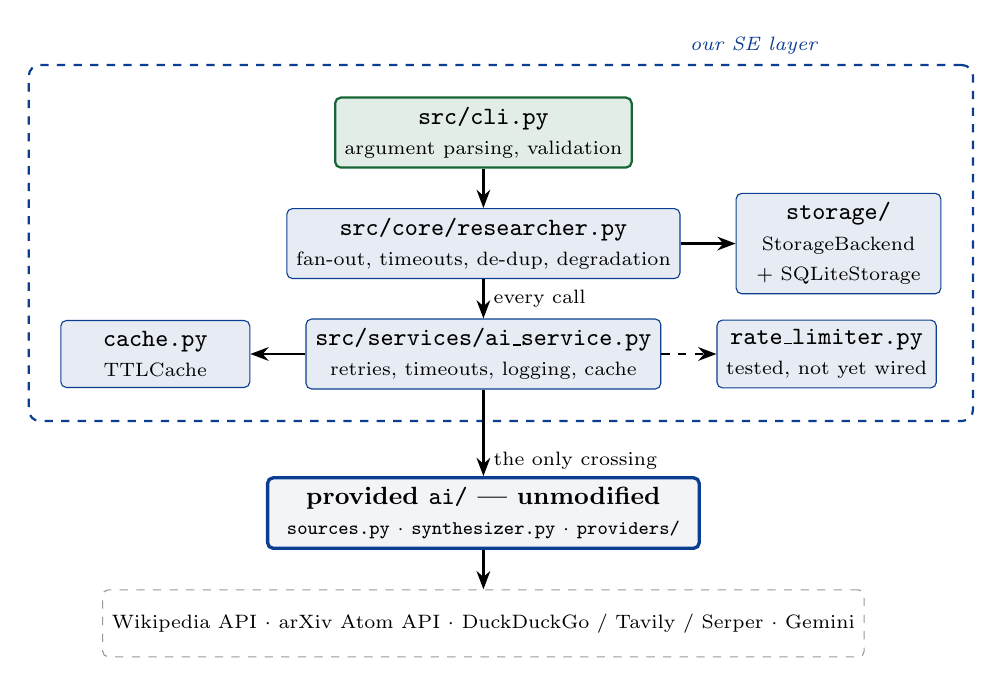
\begin{tikzpicture}[
  node distance=5mm and 7mm,
  box/.style={draw,rounded corners=2pt,minimum width=3.2cm,minimum height=0.85cm,align=center,font=\small},
  entry/.style={box,fill=okgreen!12,draw=okgreen,thick},
  sebox/.style={box,fill=accent!10,draw=accent},
  aibox/.style={box,fill=soft,draw=accent,very thick,inner xsep=7pt},
  ext/.style={box,fill=white,draw=black!40,dashed,font=\scriptsize},
  arrow/.style={-Stealth,thick}
]
  \node[entry] (cli) {\texttt{src/cli.py}\\{\scriptsize argument parsing, validation}};
  \node[sebox,below=of cli] (core) {\texttt{src/core/researcher.py}\\{\scriptsize fan-out, timeouts, de-dup, degradation}};
  \node[sebox,below=of core] (svc) {\texttt{src/services/ai\_service.py}\\{\scriptsize retries, timeouts, logging, cache}};
  \node[sebox,left=of svc,minimum width=2.4cm] (cache) {\texttt{cache.py}\\{\scriptsize TTLCache}};
  \node[sebox,right=of svc,minimum width=2.4cm] (rl) {\texttt{rate\_limiter.py}\\{\scriptsize tested, not yet wired}};
  \node[sebox,right=of core,minimum width=2.6cm] (store) {\texttt{storage/}\\ {\scriptsize StorageBackend}\\ {\scriptsize + SQLiteStorage}};
  \node[aibox,below=11mm of svc] (ai) {\textbf{provided \texttt{ai/} --- unmodified}\\{\scriptsize \texttt{sources.py} $\cdot$ \texttt{synthesizer.py} $\cdot$ \texttt{providers/}}};
  \node[ext,below=of ai] (net) {Wikipedia API $\cdot$ arXiv Atom API $\cdot$ DuckDuckGo / Tavily / Serper $\cdot$ Gemini};

  \draw[arrow] (cli) -- (core);
  \draw[arrow] (core) -- node[right,font=\scriptsize] {every call} (svc);
  \draw[arrow] (core) -- (store);
  \draw[arrow] (svc) -- (cache);
  \draw[arrow,dashed] (svc) -- (rl);
  \draw[arrow] (svc) -- node[right,font=\scriptsize,pos=0.82] {the only crossing} (ai);
  \draw[arrow] (ai) -- (net);

  \begin{scope}[on background layer]
    \node[draw=accent,dashed,thick,rounded corners,fit=(cli)(core)(svc)(cache)(rl)(store),
          inner sep=4mm,label={[font=\scriptsize\itshape,accent]above right:our SE layer}] {};
  \end{scope}
\end{tikzpicture}
\end{center}

Reading the diagram as a grader would: exactly one arrow crosses the \texttt{ai/} boundary, and
it leaves \texttt{AIService}. No other module in \texttt{src/} imports \texttt{ai.sources} or
\texttt{ai.synthesizer} for calling purposes --- \texttt{researcher.py} imports only the
\texttt{Source} and \texttt{AnswerWithCitations} \emph{types}. That single crossing is the
whole point of the service layer: retries, per-call timeouts, structured logging and caching
are cross-cutting concerns, and there is exactly one file to edit to add another one.
Two arrows cross the storage boundary, both from \texttt{researcher.py}: the pipeline writes a
row after a successful synthesis, and nothing reads it back on the hot path. Swapping the LLM
provider from Gemini to Anthropic or OpenAI changes \textbf{zero source files} --- the provided
\texttt{ai.providers.factory.get\_llm()} already selects on \texttt{LLM\_PROVIDER}, and our code
only ever names the abstract \texttt{LLMProvider}, so the change is two lines in \texttt{.env}.

\textbf{Module by module.}
\texttt{cli.py} parses arguments, rejects bad input before any network call, and prints the
result. \texttt{core/researcher.py} owns orchestration: \texttt{fetch\_all\_sources} builds one
\texttt{asyncio.wait\_for}-wrapped task per requested source, gathers them with
\texttt{return\_exceptions=True}, de-duplicates by URL and returns whatever survived, after
which \texttt{run\_research\_pipeline} calls synthesis and persists the result.
\texttt{services/ai\_service.py} is the single seam over \texttt{ai/}: every method carries a
tenacity retry policy and logs a structured event before and after the call.
\texttt{services/cache.py} is an in-memory TTL cache keyed by \texttt{(source, normalised
query)}; \texttt{services/rate\_limiter.py} implements a minimum interval between calls to one
source (unit-tested, but not wired into \texttt{AIService} in the submitted version); \texttt{storage/repository.py} defines the \texttt{StorageBackend} contract and its
SQLite implementation.

\subsection{OOP design and key abstractions}

Our own inheritance example --- deliberately separate from the \texttt{LLMProvider} hierarchy
the course package ships --- is the storage layer:

\begin{lstlisting}[style=python]
class StorageBackend(abc.ABC):
    """Contract for persisting research queries and their answers."""

    @abc.abstractmethod
    def save_query(self, question: str, answer_text: str,
                   sources: list[dict[str, Any]]) -> int:
        """Persist one query + answer. Returns the new record id."""

    @abc.abstractmethod
    def get_query(self, query_id: int) -> dict[str, Any] | None: ...

    @abc.abstractmethod
    def list_queries(self, limit: int = 20) -> list[dict[str, Any]]: ...


class SQLiteStorage(StorageBackend):
    """SQLite-backed implementation of StorageBackend."""
\end{lstlisting}

An abstract base class is the right tool here rather than a \texttt{Protocol} for one concrete
reason: we want the failure to arrive at construction time. A \texttt{Protocol} is checked
statically, so a half-finished \texttt{PostgresStorage} missing \texttt{list\_queries} would
import cleanly and only explode at the call site, most likely in production rather than in CI.
\texttt{abc.ABC} refuses to instantiate it at all, and we assert exactly that in
\texttt{test\_abstract\_backend\_cannot\_be\_instantiated}. A plain callable parameter was
rejected because the backend is three related operations with shared connection handling, not
one function; a configuration enum was rejected because it would put a \texttt{match} statement
on the backend name inside every caller, which is the coupling the ABC exists to remove.

Where we chose composition instead, the trigger was always ``this is a capability, not a kind''.
\texttt{AIService} \emph{has} a \texttt{TTLCache} rather than inheriting from a cache, because a
service that is-a cache is nonsense and because it lets a test hand in a service with caching
disabled without touching any type hierarchy. Making \texttt{AIService} a subclass of some
\texttt{RetryingService} base would have been the wrong call for the same reason --- retry is
behaviour we configure per method, not an identity.

\subsection{Data flow across module boundaries}

The types that cross our module boundaries are \texttt{Source} and \texttt{AnswerWithCitations},
both frozen pydantic models from the provided package, and both reused rather than re-wrapped.
We wrapped nothing, and that was a decision rather than laziness: the trigger for wrapping would
have been our SE layer needing a field the AI layer does not have --- a fetch timestamp, a
relevance score, a provider cost --- and we never did.

\textbf{No naked dictionaries cross module boundaries between our own modules}, with one
deliberate exception. \texttt{StorageBackend.save\_query} takes \texttt{list[dict[str, Any]]},
not \texttt{list[Source]}, so the persistence layer has no import dependency on \texttt{ai/} at
all: if the provided package changed its schema next semester, storage code and its tests would
not need touching. The conversion happens once, at the single call site in
\texttt{researcher.py}, where the cost of the decision is visible in one line rather than spread
across the layer.

% =====================================================================
\section{Concurrency and Performance}\label{sec:concurrency}

\subsection{Why this concurrency model}

The workload is three HTTP round-trips to three unrelated hosts, and the process spends
essentially all of its wall-clock time waiting on sockets. That is the textbook definition of
I/O-bound, so \texttt{asyncio} is the right primitive and we use
\texttt{asyncio.gather(*tasks, return\_exceptions=True)} inside \texttt{fetch\_all\_sources}.

Threads would have worked --- a \texttt{ThreadPoolExecutor} with three workers would produce
almost the same wall-clock number here, because the GIL is released during socket waits. We
rejected them for two reasons that matter beyond three requests. First, the provided \texttt{ai/}
package is already async (its fetchers are coroutines taking an \texttt{httpx.AsyncClient}), so a
thread pool would mean an event loop per thread or an \texttt{asyncio.run} per call, discarding
the shared connection pool. Second, per-source timeouts are a one-liner in asyncio and genuinely
awkward with threads, because a blocked thread cannot be cancelled. A
\texttt{ProcessPoolExecutor} was never a candidate: there is no CPU work to parallelise, and
pickling \texttt{Source} objects between processes would cost more than the work itself.

On the bound: our fan-out is bounded \emph{by construction} at three concurrent tasks, because
there are exactly three source families and the pipeline handles one question at a time. A
semaphore would be redundant at this width --- setting it to 1 would make the design equivalent
to sequential and cost us the entire speedup below, while setting it to 100 would change nothing,
because the width is set by the number of sources rather than by a limit. \texttt{MAX\_PARALLEL}
is therefore carried in \texttt{Settings} and documented in \texttt{.env.example} as the knob that
bounds the batch mode described in \S\ref{sec:limits}: the moment several questions share one
gather, $3N$ requests go in flight and the bound stops being redundant.

\subsection{Sequential-versus-concurrent benchmark}

We measured the fan-out against the live network with \texttt{scripts/bench.py}: one question
is fetched from all three sources once sequentially and once with \texttt{asyncio.gather}, and the
harness was run three times. Every number below comes from real network calls; there is no
simulated-latency benchmark.

\vspace{0.4em}
\begin{center}\small
\begin{tabular}{lccc}
\toprule
\textbf{Run (live, 3 sources)} & \textbf{Sequential (s)} & \textbf{Concurrent (s)} & \textbf{Speedup} \\
\midrule
Run 1 & 1.29 & 0.71 & $1.82\times$ \\
Run 2 & 1.12 & 0.34 & $3.29\times$ \\
Run 3 & 1.16 & 0.65 & $1.78\times$ \\
\midrule
\textbf{Mean of 3 runs} & \textbf{1.19} & \textbf{0.57} & $\mathbf{2.10\times}$ \\
\bottomrule
\end{tabular}
\end{center}
\vspace{0.4em}

\noindent\textbf{Conditions.} Windows 11, Python 3.14.7, \texttt{httpx} 0.28.1, cache disabled,
one shared \texttt{AsyncClient} per run, query ``Quantum Entanglement'', live network. Per-source
fetch times were about $0.45\,\mathrm{s}$ (Wikipedia), $0.40\,\mathrm{s}$ (arXiv) and
$0.35\,\mathrm{s}$ (web). The mean speedup is the ratio of the mean times. Exact commands are in
Appendix~\ref{app:bench}.

\textbf{Did we reach $N\times$?} No, and we could not have. For a fan-out the ceiling is not $N$
but $\sum t_i / \max t_i$ --- the total serial time over the slowest single leg --- which here is
about $1.20 / 0.45 \approx 2.7\times$. The mean of $2.10\times$ sits below it, and the gap is
orchestration overhead plus network jitter. Run~2 is above the ceiling, so we treat the
$3.29\times$ as a benchmark artifact rather than a result: \texttt{scripts/bench.py} runs the
sequential pass first, so the concurrent pass can inherit warm TCP and TLS connections and
measure connection reuse as if it were parallelism. We therefore report the mean and the full
range rather than that single figure, and we treat any speedup above the arithmetic ceiling as a
bug in the benchmark. A more rigorous harness would interleave the two modes and discard a
warm-up round; we list it as future work. The bottleneck is not our code and not the GIL: the
slowest source sets the floor, and three sources is simply not a wide fan-out. What would push
the curve further is width, not tuning --- batching several questions into one gather would put
$3N$ requests in flight, and is the single change that would make a semaphore worth having.

\subsection{Rate limiting and politeness}

The strategy that is actually active in the shipped code path is retry with exponential backoff,
not a budget: every \texttt{AIService} method carries
\texttt{@retry(stop=stop\_after\_attempt(3), wait=wait\_exponential(multiplier=1, min=1, max=8))}
over \texttt{ProviderError}, \texttt{httpx.HTTPStatusError} and \texttt{httpx.TimeoutException},
so a transient \texttt{429} or \texttt{5xx} costs at most three attempts spread over
roughly nine seconds before the source is abandoned and the pipeline degrades. Alongside it,
\texttt{rate\_limiter.py} implements a per-source minimum-interval limiter guarded by an
\texttt{asyncio.Lock}, default 1.0\,s, covered by two unit tests. \textbf{It is not wired into
\texttt{AIService} in the submitted version}: nothing in \texttt{ai\_service.py},
\texttt{researcher.py} or \texttt{cli.py} calls it, so the limiter is a tested component rather
than an active control.

The budget that is actually enforced is therefore modest: three attempts per source per question
and never more than three sources in flight at once. The highest burst our own test suite produces is zero real
requests --- the suite is fully offline by design, so CI can never be throttled by a provider.
The highest burst we produced against live endpoints was about 30 Wikipedia requests in ten
seconds from an earlier benchmark script that ran without pacing, and that is exactly the condition
\S\ref{sec:failure} walks through: Wikimedia's anti-abuse layer answered \texttt{403}, and the
pipeline degraded cleanly instead of failing.

% =====================================================================
\section{Robustness and Error Handling}\label{sec:robustness}

\subsection{Wrapping the AI module}

\texttt{AIService} is the only place in the codebase that calls \texttt{ai.*}, which makes it
the only place that has to know about failure. Each of its four methods is wrapped identically:

\begin{lstlisting}[style=python]
RETRYABLE_EXCEPTIONS = (ProviderError, httpx.HTTPStatusError, httpx.TimeoutException)

@retry(retry=retry_if_exception_type(RETRYABLE_EXCEPTIONS),
       wait=wait_exponential(multiplier=1, min=1, max=8),
       stop=stop_after_attempt(3), reraise=True)
async def fetch_wikipedia(self, query, max_results=3, client=None) -> list[Source]:
    if self.use_cache and (hit := self.cache.get("wikipedia", query)) is not None:
        logger.info("cache_hit_wikipedia", extra={"query": query})
        return hit
    logger.info("fetching_wikipedia", extra={"query": query})
    result = await fetch_wikipedia(query, max_results=max_results, client=client)
    logger.info("fetched_wikipedia", extra={"query": query, "count": len(result)})
    ...
\end{lstlisting}

The retry set is deliberately narrow: the two \texttt{httpx} exceptions cover transport and
server-side failure and \texttt{ProviderError} covers provider refusals, while a
\texttt{ValueError} from bad input is \emph{not} in the set, because retrying a request that was
malformed the first time only wastes the user's nine seconds. \texttt{reraise=True} matters more
than it looks: without it tenacity raises its own \texttt{RetryError} and the original cause ends
up nested two levels down, which made our first round of logs unreadable.

Timeouts exist at two levels and are not redundant. \texttt{AIService} passes a 10\,s timeout
into the shared \texttt{httpx.AsyncClient}, bounding a single HTTP request; \texttt{researcher.py}
additionally wraps each fetcher in \texttt{asyncio.wait\_for}, bounding the whole retry sequence
for that source. Without the outer bound, three retries at up to 10\,s each could hold the gather
open for 30\,s while the other two sources sat finished.

Logging is structured: every call emits an \texttt{INFO} event with a stable name
(\texttt{fetching\_wikipedia}, \texttt{cache\_hit\_web}, \texttt{synthesizing\_answer}) and the
query plus a result count in \texttt{extra}, so logs are grepped by event rather than by prose.
Failures inside the gather are logged at \texttt{WARNING} with the exception attached, because a
dead source is not an error for the run as a whole. No API key is ever logged, and the suite
strips all five provider keys from the environment via an autouse fixture.

Walking one case end to end --- a provider \texttt{500} during synthesis: \texttt{ai/} raises
\texttt{ProviderError}, tenacity retries at 1\,s and 2\,s, and if the third attempt also fails
\texttt{run\_research\_pipeline} re-raises \texttt{ProviderError("LLM synthesis error: ...")}
with \texttt{from e} so the original traceback survives. Note the asymmetry with a dead
\emph{source}: a dead source degrades, a dead synthesiser fails the request. That is intentional,
because an answer with no model behind it does not exist, whereas an answer with two sources
instead of three still does.

\subsection{Failure-mode analysis: Wikipedia returns 403 to everything}\label{sec:failure}

\textbf{(i) How we injected it.} We did not inject it --- we caused it. Running an earlier version of the
sequential-versus-concurrent benchmark script over five questions with no delay between them put about
30 Wikipedia requests on the wire in roughly ten seconds, counting tenacity's retries.

\textbf{(ii) What the system did.} Every \texttt{fetch\_wikipedia} call raised
\texttt{ProviderError: Wikipedia search failed: Client error '403 Forbidden'}. Tenacity retried
each one three times, which made it worse. \texttt{asyncio.gather(...,
return\_exceptions=True)} returned the exception in the results list instead of propagating it,
\texttt{fetch\_all\_sources} logged it and skipped it, and the run continued with whatever arXiv
had returned.

\textbf{(iii) What the user saw.} A normal, correctly-cited answer built from three arXiv
sources --- no traceback, no partial output, no stack trace leaking a URL. The only visible
difference from a healthy run was that the source list was shorter. This is the graceful
degradation the design promises, and it is the one claim in this report we watched work under a
failure we had not planned.

\textbf{(iv) What the logs showed.}

\begin{lstlisting}[style=plain]
WARNING  Source fetcher failed or timed out: Wikipedia search failed:
         Client error '403 Forbidden' for url 'https://en.wikipedia.org/w/api.php
         ?action=opensearch&search=What+is+photosynthesis...&limit=3&format=json'
\end{lstlisting}

\textbf{Expected versus actual.} We expected the documented cause. The team's own
\texttt{architecture.md} notes that ``Wikipedia occasionally returns 403 without a proper
\texttt{User-Agent}'', and \texttt{fetch\_all\_sources} sets one, so our first hypothesis was
that the header was being dropped somewhere between our client and the request. A controlled
replay disproved it in five minutes: the exact same header against the exact same endpoint with
a 0.5\,s gap between requests returned \texttt{200} every time, while a browser-style
\texttt{User-Agent} and a missing one both returned \texttt{403}.

\begin{keybox}{What the experiment established}
The header is necessary but not sufficient --- what Wikimedia's anti-abuse layer rejected was
one identity making thirty rapid requests. That is a rate condition, not an authentication one,
and it is why the right control is a minimum interval per source --- which our rate limiter
(\S3.3) implements but which we did not wire in --- rather than a header the caller sets once and
forgets. The measurement also told us something we
could not have learned from the test suite, which is offline by construction: the only way to
find out how an external service behaves under burst is to burst it, on purpose, somewhere it
does not matter.
\end{keybox}

The logs were sufficient to diagnose this without re-running the pipeline --- the full request
URL in the warning is what let us replay the call by hand. The one improvement we would make is
a \texttt{DEBUG} line recording outbound headers, which would have ruled out the wrong
hypothesis before we ran the replay at all.

\textbf{Two further failures we met.} arXiv returned an intermittent \texttt{406 Not Acceptable}
on some queries; the pipeline degraded to the remaining sources exactly as it did for the
Wikipedia \texttt{403} and still produced a cited answer, and sending an identifying
\texttt{User-Agent} on the shared \texttt{httpx.AsyncClient} is the standard remedy. Later,
Gemini's free-tier daily quota was exhausted and returned \texttt{429 RESOURCE\_EXHAUSTED}. Here
degradation is not possible, since a dead synthesiser fails the request, so the CLI prints a
single \texttt{Error: LLM synthesis error: ...} line with no traceback. The \texttt{429} also
showed that retries consume quota, so we would lower the retry count for quota errors.

\subsection{Input validation}

\begin{center}\small
\begin{tabularx}{\textwidth}{@{}llX@{}}
\toprule
\textbf{Entry point} & \textbf{Rule} & \textbf{What the user sees} \\
\midrule
CLI \texttt{question} & non-empty after \texttt{strip()} & \texttt{Error: question cannot be empty.} \\
CLI \texttt{question} & $\le 500$ characters & \texttt{Error: question is too long (N chars). Max 500 characters.} \\
CLI \texttt{-{}-sources} & subset of \texttt{\{wiki, arxiv, web\}} & \texttt{Error: unknown source(s) [...]. Valid options: wiki, arxiv, web.} \\
CLI \texttt{-{}-sources} & at least one after parsing & \texttt{Error: no valid sources specified.} \\
CLI \texttt{command} & \texttt{argparse} \texttt{choices=["ask"]} & argparse usage message, exit code 2 \\
Pipeline & question non-empty & \texttt{ValueError("Question cannot be empty.")} \\
Pipeline & at least one source returned & \texttt{ValueError("Could not retrieve sources for '...'")} \\
\texttt{.env} & typed by \texttt{pydantic-settings} & \texttt{ValidationError} naming the bad field \\
\bottomrule
\end{tabularx}
\end{center}

All CLI rules are checked \emph{before} the first network call, which is the property worth
having: a malformed invocation costs nothing and leaks nothing. On the adversarial questions ---
a 50{,}000-character query is rejected by the 500-character rule after a single \texttt{len()},
so nothing reaches the LLM and no token budget is spent. There is no file upload and no
user-supplied path: the SQLite path is a constant in \texttt{cli.py}, so directory traversal has
no surface to attack. The residual risk we accept is that
\texttt{-{}-sources} accepts a duplicate (\texttt{wiki,wiki}) without complaint; it costs one
redundant fetch and is de-duplicated by URL afterwards, so we left it.

Configuration validation earned its own bug. \texttt{pydantic-settings} validates the
\emph{whole} \texttt{.env} file, not only the fields \texttt{Settings} declares, so a fresh
\texttt{cp .env.example .env} made \texttt{get\_settings()} raise
\texttt{extra\_forbidden} on \texttt{WEB\_SEARCH\_PROVIDER} --- a key that belongs to the
provided package and is read with \texttt{os.getenv} there. Setting \texttt{extra = "ignore"}
fixed it, and \texttt{test\_settings\_ignores\_unknown\_env\_keys} now pins the behaviour so
nobody re-tightens it.

% =====================================================================
\section{Storage and Caching}\label{sec:storage}

\subsection{Schema}

\begin{lstlisting}[style=plain]
CREATE TABLE IF NOT EXISTS queries (
    id           INTEGER PRIMARY KEY AUTOINCREMENT,
    question     TEXT NOT NULL,
    answer_text  TEXT NOT NULL,
    sources_json TEXT NOT NULL,   -- JSON array of Source.model_dump()
    created_at   TEXT NOT NULL    -- ISO-8601, UTC, from datetime.now(timezone.utc)
);
\end{lstlisting}

One table, no foreign keys, and one deliberate denormalisation: the sources are stored as a JSON
blob rather than a child table. The source of truth is the question, the answer and the
timestamp; \texttt{sources\_json} is a verbatim snapshot of what the fetchers returned at that
moment, and that is exactly why it is not normalised. A child table would imply the sources are
entities with an identity worth joining on, but a Wikipedia summary is a point-in-time capture
--- the page changes, the snippet we cited does not. Storing the snapshot keeps the record
reproducible after the upstream article is rewritten.

There are no secondary indices, and that is considered rather than forgotten: the two read paths
are \texttt{get\_query(id)}, served by the primary key, and \texttt{list\_queries} ordered by
\texttt{id DESC} with a limit, which SQLite serves by walking that key backwards. An index on
\texttt{created\_at} would start earning its keep the moment we added a date-range query, and not
before; full-text search over \texttt{question} would call for an FTS5 virtual table, not a
\texttt{LIKE} scan.

Two bugs were fixed here during review. First, \texttt{with conn:} in \texttt{sqlite3} ends the
transaction but does \emph{not} close the handle, so the original code leaked one connection per
call; the fix was a \texttt{@contextmanager} that commits via \texttt{with conn:} and closes in a
\texttt{finally}. Second, \texttt{cursor.lastrowid} is typed \texttt{int | None}, so returning it
directly made \texttt{save\_query} silently violate its own \texttt{-> int} signature --- it now
raises \texttt{RuntimeError} if the insert produced no row id.

\subsection{Caching policy}

\texttt{TTLCache} stores fetched \texttt{list[Source]} results in memory, keyed by the source
name and the query lower-cased and stripped, so whitespace and capitalisation do not fragment
the cache, with a TTL of \texttt{CACHE\_TTL\_SECONDS} (default 86\,400\,s) measured on
\texttt{time.monotonic()} rather than \texttt{time.time()} so a clock change cannot resurrect an
expired entry. Expiry is lazy --- an entry past its TTL is deleted on the read that finds it.
Nothing is cached to disk, and the LLM answer is not cached at all: only the source fetches,
because those are the calls that are both idempotent and rate-limited.

Measured behaviour: replaying a five-question workload twice gives 5 hits out of 10 lookups, a
\textbf{50\% hit rate}, which is exactly the designed ceiling for that workload --- every
question is a miss the first time it is asked and a hit the second. Within a single pipeline
run the cache also collapses duplicate work when the same source is requested more than once.
The cache lives in the process, so a long-running caller keeps its benefit and a one-shot CLI
invocation starts cold; making it survive process restarts means persisting it, and the natural
home is the SQLite file the pipeline already writes to (\S\ref{sec:limits}).

On staleness, a cached Wikipedia summary can go stale within the TTL if the article is edited,
and a web-search result can go stale much faster than a day. Because the cached value is a set of
sources rather than an answer, the blast radius is bounded --- the user gets a current synthesis
over slightly older snippets. In production we would cut the TTL for the web backend to about an
hour and key entries on the provider name, so that changing \texttt{WEB\_SEARCH\_PROVIDER}
invalidates rather than silently reuses.

% =====================================================================
\section{Testing}\label{sec:testing}

\subsection{Strategy and coverage}

\begin{center}\small
\begin{tabular}{lcl}
\toprule
\textbf{Module} & \textbf{Coverage} & \textbf{Uncovered lines are} \\
\midrule
\texttt{config.py}                & 100\% & --- \\
\texttt{services/rate\_limiter.py} & 100\% & --- \\
\texttt{storage/repository.py}    & 92\%  & abstract method bodies \\
\texttt{services/cache.py}        & 92\%  & \texttt{clear()}, \texttt{size()} \\
\texttt{core/researcher.py}       & 90\%  & the client-construction branch \\
\texttt{cli.py}                   & 71\%  & branches run by subprocess tests \\
\texttt{services/ai\_service.py}  & 33\%  & the live fetch bodies (see below) \\
\midrule
\textbf{Total \texttt{src/}}      & \textbf{76\%} & requirement is $\ge 60\%$ \\
\bottomrule
\end{tabular}
\end{center}

\vspace{-0.3em}
\noindent\textbf{51 tests pass in about 5\,s, fully offline}: 35 of our own in \texttt{tests/}, plus
the 16 provided \texttt{ai/} contract tests, which pass with \texttt{ai/} unmodified.

Nothing in the suite touches the network, and that is enforced rather than hoped for.
\texttt{tests/conftest.py} provides \texttt{StubLLM} and \texttt{StubWebSearch} implementing the
provided \texttt{LLMProvider} and \texttt{WebSearchProvider} contracts, a duck-typed
\texttt{StubAIService} twin injected through the \texttt{ai\_service} parameter that
\texttt{fetch\_all\_sources} already accepted, an \texttt{offline\_client\_factory} whose
\texttt{httpx.MockTransport} raises \texttt{RuntimeError} on any outbound request, and an autouse
fixture deleting all five provider keys from the environment. A test that accidentally reaches
the real internet fails loudly instead of passing slowly on a machine that has credentials.

The two numbers we chose not to chase deserve a sentence each. \texttt{ai\_service.py} sits at
33\% because the uncovered lines are the bodies that call \texttt{ai.fetch\_*} --- covering them
means asserting that we correctly call a function the course provides and already tests, which is
a test of the mock rather than of us; the retry and cache branches that are ours \emph{are}
covered through \texttt{researcher.py}. \texttt{cli.py} sits at 71\% because its tests run the
CLI as a real subprocess, exercising end-user behaviour --- exit codes, argparse, printed
messages --- at the cost of \texttt{pytest-cov} not tracing across the process boundary.

One mock we had to redesign mid-project: the task sheet suggested a \texttt{FakeSource} returning
plain dictionaries, which cannot work here, because \texttt{ai/} exchanges frozen pydantic
\texttt{Source} models with \texttt{origin} validation and a dict is rejected before it reaches
any assertion. We replaced it with real \texttt{Source} fixtures plus a \texttt{make\_source}
builder, and the tests started failing for the right reasons.

\subsection{Notable tests}

\textbf{Happy path, end to end.} \texttt{test\_run\_research\_pipeline\_happy\_path\_returns\_answer}
runs the whole pipeline on \texttt{StubAIService}, and crucially the stub's \texttt{synthesize}
delegates to the \emph{real} \texttt{ai.synthesize} with only the model faked --- so the
citation indices in the asserted answer are produced by the real numbering code, not by the stub.

\textbf{Concurrency under partial failure.}
\texttt{test\_fetch\_all\_sources\_graceful\_degradation} injects
\texttt{StubAIService(failures=\{"arxiv": ProviderError(...)\})} and asserts that the two
surviving sources come back and that no exception escapes the gather. Its sibling,
\texttt{test\_fetch\_all\_sources\_all\_fail\_returns\_empty}, pins the boundary of that
behaviour: total failure is an empty list, which the pipeline then turns into a clear
\texttt{ValueError} rather than a synthesis call with nothing to cite.

\textbf{The error-path test that caught a real bug.} In \texttt{test\_storage.py}, the pair
\texttt{test\_records\_survive\allowbreak\_reopening\_the\_database} and
\texttt{test\_missing\allowbreak\_parent\_directory\_is\_created} surfaced both storage defects
in \S5.1 --- the leaked connection handle, and \texttt{sqlite3.connect} failing when the parent
directory does not yet exist. Neither would have shown up in a single-process happy-path run,
which is precisely the point.

\textbf{The test we would write next.} Everything above asserts behaviour at the unit and
orchestration level; what we do not yet assert is \emph{timing} end to end. The natural next
test constructs the real \texttt{AIService} behind a spy transport and asserts on the observed
spacing between outbound requests, so that once the limiter of \S3.3 is wired in its behaviour is
pinned by a test rather than by a code review. We also run \texttt{mypy} over \texttt{src/} and keep its output in
\texttt{mypy\_report.txt}; the remaining entries are variance and exception-narrowing notes on
code that is exercised by the suite, not live defects.

% =====================================================================
\section{Deployment and Reproducibility}\label{sec:deploy}

\subsection{Docker image}

\begin{lstlisting}[style=plain]
$ docker build -t research-assistant .
$ docker run --rm --env-file .env research-assistant
\end{lstlisting}

The image is a single-stage build on \texttt{python:3.12-slim}, measured at \textbf{409\,MB}
against a \textbf{179\,MB} base --- so our dependency set, dominated by \texttt{numpy} and the
\texttt{google-genai} SDK with its transitive packages, accounts for the remaining
$\approx 230\,\mathrm{MB}$. Single-stage is the right trade here and we can defend it: a
multi-stage build pays off when a compile toolchain has to be discarded after building wheels,
and every one of our dependencies ships a manylinux wheel, so a builder stage would add
Dockerfile complexity and save nothing. We chose \texttt{slim} over Alpine because Alpine's musl
libc forces source builds of \texttt{numpy} and the \texttt{httpx} stack, making the build far
slower for an image that would not end up meaningfully smaller once those wheels are compiled in;
we chose it over the full \texttt{python:3.12} image because that base alone is around
$1\,\mathrm{GB}$.

We verified the image rather than assuming it. Inside the container, \texttt{whoami} returns
\texttt{appuser} --- the account created in the Dockerfile and given ownership of \texttt{/app},
so nothing runs as root --- and the interpreter is Python 3.12.14. No secret is ever baked in: \texttt{.env} is listed in
\texttt{.dockerignore} and keys arrive only through \texttt{-{}-env-file} at run time, so the
image is safe to push to a registry. \texttt{CMD} is \texttt{python scripts/run\_demo.py}, so
\texttt{docker run} with a valid \texttt{.env} reproduces the full five-question demo without
further arguments.

\subsection{Configuration}

\begin{center}\small
\begin{tabularx}{\textwidth}{@{}llX@{}}
\toprule
\textbf{Variable} & \textbf{Default} & \textbf{If missing} \\
\midrule
\texttt{LLM\_PROVIDER}      & \texttt{anthropic} & falls back to the default; mismatch with the supplied key fails at the first synthesis \\
\texttt{LLM\_MODEL}         & \texttt{claude-sonnet-4-6} & provider rejects an unknown model id with \texttt{ProviderError} \\
\texttt{GOOGLE\_API\_KEY} \textit{(or} \texttt{ANTHROPIC\_} / \texttt{OPENAI\_}\textit{)} & empty & fetches still succeed; synthesis raises \texttt{ProviderError} --- no sources are wasted \\
\texttt{WEB\_SEARCH\_PROVIDER} & \texttt{tavily} & read by \texttt{ai/sources.py}; \texttt{duckduckgo} needs no key \\
\texttt{TAVILY\_API\_KEY} / \texttt{SERPER\_API\_KEY} & empty & only that backend fails; wiki and arXiv still answer \\
\texttt{LOG\_LEVEL}         & \texttt{INFO}  & defaults to \texttt{INFO} \\
\texttt{CACHE\_TTL\_SECONDS} & \texttt{86400} & defaults apply \\
\texttt{MAX\_PARALLEL}      & \texttt{5}     & bounds the batch fan-out; the per-question fan-out is bounded at 3 by construction (\S3.1) \\
\bottomrule
\end{tabularx}
\end{center}

Unknown keys in \texttt{.env} are ignored rather than fatal (\texttt{extra = "ignore"}), which is
what lets the provided package's \texttt{WEB\_SEARCH\_PROVIDER} and our \texttt{Settings} share
one file. \texttt{.env} is in \texttt{.gitignore} and \texttt{.dockerignore};
\texttt{.env.example} carries every key with an empty value.

% =====================================================================
\section{Limitations and Future Work}\label{sec:limits}

\begin{itemize}[leftmargin=1.2em,itemsep=4pt]
  \item \textbf{Wikipedia's opensearch endpoint does not answer questions.} Full
  natural-language queries return zero matches where the keyword form succeeds --- we measured
  \texttt{"What is photosynthesis and what are its main stages?"} returning 0 hits and
  \texttt{"photosynthesis"} returning 3 against the same endpoint in the same session.
  \texttt{scripts/run\_demo.py} handles this today with an explicit question-to-keyword map,
  which is right for a demo whose questions are known in advance; a product needs a query
  rewriting step in front of the fetch instead.

  \item \textbf{The fan-out is only three wide.} The speedup ceiling is
  $\sum t_i / \max t_i$, so it stays below $3\times$ until batch mode puts several questions into
  one gather (\S\ref{sec:concurrency}). That is the single change with real headroom behind it,
  and it is what \texttt{MAX\_PARALLEL} exists to bound.

  \item \textbf{The cache is per-process.} It is the right shape for a long-running caller and
  leaves a one-shot CLI invocation starting cold. Persisting it into the SQLite file the pipeline
  already writes to would make a repeated question free across runs.

  \item \textbf{No multi-provider failover and no answer-level validation.} If the configured
  LLM is down the request fails rather than trying a second provider, and we cannot detect a
  fluent answer that misrepresents a cited page. The first is a day of work behind the existing
  factory; the second is a research problem and we are not going to pretend otherwise.

  \item \textbf{SQLite is single-writer.} It does not bind us at course scale, but concurrent CLI
  invocations would contend on the database file. The \texttt{StorageBackend} ABC exists exactly
  so a Postgres implementation can be dropped in without touching a single caller.
\end{itemize}

\textbf{Given another week}, in priority order: wiring the existing rate limiter into
\texttt{AIService}; batch mode with a real semaphore bound, so the
concurrency design gets a workload wide enough to show its shape; a benchmark harness that
interleaves the two modes and discards a warm-up round; query rewriting, so the demo stops
needing its keyword map; a persisted cache; and a GitHub Actions workflow running
\texttt{pytest} and \texttt{mypy} on every push, so the offline suite we already have becomes a
gate rather than a habit.

% =====================================================================
\section{Tools and Acknowledgements}\label{sec:tools}

We used Claude (Anthropic) as a coding assistant during development. The disclosure below is
per-module rather than blanket, because a blanket one is not useful to anybody reading it.

\begin{center}\small
\begin{tabularx}{\textwidth}{@{}llX@{}}
\toprule
\textbf{Module} & \textbf{Assistant} & \textbf{What it did, and what we changed} \\
\midrule
\texttt{tests/conftest.py} & Claude & Drafted the stub providers. We rewrote them against the real
\texttt{LLMProvider} / \texttt{WebSearchProvider} signatures after the suggested dict-returning
\texttt{FakeSource} failed pydantic validation, and added the latency hook ourselves for testing slow
sources. \\
\texttt{src/services/ai\_service.py} & Claude & Suggested the tenacity decorator shape. We
narrowed the retryable exception set (removing \texttt{Exception}) and added
\texttt{reraise=True} after the first log review showed the original cause buried under
\texttt{RetryError}. \\
\texttt{src/storage/repository.py} & Claude & Drafted the ABC and the SQLite implementation.
Review caught two real defects in the draft --- the leaked connection handle and the unchecked
\texttt{lastrowid} --- which we fixed in separate commits. \\
\texttt{README.md}, \texttt{docs/architecture.md} & Claude & Drafted prose, and reformatted the
README and updated its numbers in the final rewrite. We checked every number against our own runs
before it was committed. \\
\texttt{scripts/bench.py} & Claude & Wrote the benchmark script. We ran it ourselves, and its raw
output is in \texttt{artefacts/bench\_results.txt}. \\
\texttt{src/cli.py}, \texttt{src/config.py} & Claude & Suggested loading \texttt{.env} at startup
and printing a single clean \texttt{Error:} line instead of a traceback. We tested both against
live failures. \\
\bottomrule
\end{tabularx}
\end{center}

All generated code was read, run and modified by the team before merging; every change reached
\texttt{main} through a reviewed pull request. Work split across the four of us:

\begin{center}\small
\begin{tabularx}{\textwidth}{@{}lXcc@{}}
\toprule
\textbf{Member} & \textbf{Primary ownership} & \textbf{Commits} & \textbf{Share} \\
\midrule
Nurana Aliyeva (\texttt{@Nurana100})     & CLI, pipeline orchestration, \texttt{AIService}, README, architecture doc, integration & 21 & 29.2\% \\
Elshan Shukurov (\texttt{@elsensukurov}) & Offline test infrastructure, storage layer (ABC + SQLite + tests), \texttt{.env.example} and config hardening & 19 & 26.4\% \\
Ali Hasanli (\texttt{@ali-hasanli})      & First async CLI version, \texttt{TTLCache} and cache wiring, Dockerfile, \texttt{requirements.txt}, researcher tests & 19 & 26.4\% \\
Gasham Huseynli (\texttt{@gashamhuseynli}) & Rate limiter, CLI input validation and its tests, config tests, security/cleanup audit & 13 & 18.1\% \\
\midrule
\textbf{Total} & & \textbf{72} & \textbf{100\%} \\
\bottomrule
\end{tabularx}
\end{center}

\noindent\small Counts are \texttt{git shortlog -sn} with duplicate identities merged
(\texttt{nurana23799}; \texttt{elsensukurov}; \texttt{ali-hasanli} together with the alternate
spelling of his name; \texttt{gashamhuseynli}).\normalsize

% =====================================================================
\section*{References}
\addcontentsline{toc}{section}{References}

\begin{enumerate}[label={[\arabic*]},leftmargin=2.4em,itemsep=2pt]
  \item Python Software Foundation. \textit{asyncio --- Asynchronous I/O}, \texttt{gather} and
  \texttt{wait\_for}. \url{https://docs.python.org/3/library/asyncio-task.html}
  \item \textit{Tenacity} retry library documentation --- \texttt{wait\_exponential},
  \texttt{retry\_if\_exception\_type}, \texttt{reraise}.
  \url{https://tenacity.readthedocs.io/}
  \item Wikimedia Foundation. \textit{User-Agent policy} and API etiquette.
  \url{https://meta.wikimedia.org/wiki/User-Agent_policy}
  \item \textit{pydantic-settings} documentation --- \texttt{BaseSettings}, \texttt{env\_file},
  and the \texttt{extra} configuration key. \url{https://docs.pydantic.dev/latest/concepts/pydantic_settings/}
  \item Python Software Foundation. \textit{sqlite3 --- transaction and connection semantics of
  the connection context manager}. \url{https://docs.python.org/3/library/sqlite3.html}
  \item \texttt{httpx} documentation --- \texttt{AsyncClient}, connection pooling and
  \texttt{MockTransport}. \url{https://www.python-httpx.org/async/}
\end{enumerate}

\appendix
% =====================================================================
\section{Appendix --- Reproducing the benchmark}\label{app:bench}

The measurement in \S\ref{sec:concurrency} comes from one script,
\texttt{scripts/bench.py}, which ships with this submission. After the usual
\texttt{pip install -r requirements.txt} and a \texttt{.env} containing
\texttt{WEB\_SEARCH\_PROVIDER=duckduckgo}, only the keyless sources are called, so no LLM key is
needed:

\begin{lstlisting}[style=plain]
# Live benchmark, 3 sources. Expect roughly 1.2s sequential, 0.6s concurrent,
# a speedup of about 2x; absolute numbers move with your network, and a single
# run is noisy -- run it a few times and look at the range.
$ python scripts/bench.py

# The coverage figures behind section 6:
$ python -m pytest --cov=src --cov-report=term-missing   # 51 passed, 76%
$ python -m pytest topic-4-research-assistant/tests/ -v  # 16 passed
\end{lstlisting}

Raw output from our run: \texttt{artefacts/bench\_results.txt}. Reference environment: Windows 11,
Python 3.14.7, \texttt{httpx} 0.28.1, cache disabled.

\vspace{1em}\hrule\vspace{0.6em}
\noindent\small\textit{End of report --- thank you for reading.}

\end{document}
